\chapter{Espace de James $\James{p}$}\label{chapter_james}

Jusque maintenant, on a d�montr� des propri�t�s et th�or�mes tr�s diversifi�s concernant les espaces r�flexifs. Cependant, on a �vit� une question qui est rest�e ouverte pendant longtemps: est-il suffisant d'�tre isom�trique � son bidual pour qu'un espace soit r�flexif? Ce pr�sent chapitre a pour but de pr�senter un espace atypique qui a r�pondu � cette question par la n�gative. Cet espace, nomm� espace de James (en l'honneur de celui qui l'a d�couvert, Robert Clarke James), est isom�trique � son bidual, mais n'est pourtant pas r�flexif.

Pour �tre exact, nous ne verrons pas l'espace de James tel qu'il a �t� d�couvert, mais plut�t une classe d'espaces qui le contient, et pour laquelle chaque espace est non r�flexif mais isom�trique � son bidual. Cela dit, on dira que tous ces espaces sont �galement des espaces de James, vu leur forte ressemblance avec celui que James a pr�sent�. Comme il l'a fait, nous proc�derons en deux �tapes: on construit un espace non r�flexif, isomorphe � son bidual et dont l'image par l'injection canonique est de codimension 1, ensuite on change la norme pour une �quivalente plus compliqu�e mais qui rend l'espace isom�trique � son bidual.

Jusque maintenant, on a d�montr� des propri�t�s et th�or�mes tr�s diversifi�s concernant les espaces r�flexifs. Cependant, on a �vit� une question qui est rest�e ouverte pendant longtemps: est-il suffisant d'�tre isom�trique � son bidual pour qu'un espace soit r�flexif? Ce pr�sent chapitre a pour but de pr�senter un espace atypique qui a r�pondu � cette question par la n�gative. Cet espace, nomm� espace de James (en l'honneur de celui qui l'a d�couvert, Robert Clarke James), est isom�trique � son bidual, mais n'est pourtant pas r�flexif.

Pour �tre exact, nous ne verrons pas l'espace de James tel qu'il a �t� d�couvert, mais plut�t une classe d'espaces qui le contient, et pour laquelle chaque espace est non r�flexif mais isom�trique � son bidual. Cela dit, on dira que tous ces espaces sont �galement des espaces de James, vu leur forte ressemblance avec celui que James a pr�sent�. Comme il l'a fait, nous proc�derons en deux �tapes: on construit un espace non r�flexif, isomorphe � son bidual et dont l'image par l'injection canonique est de codimension 1, ensuite on change la norme pour une �quivalente plus compliqu�e mais qui rend l'espace isom�triue � son bidual.

\section{D�finition de $\James{p}$}

� partir de maintenant, et jusqu'� la fin de ce chapitre, on fixe le r�el $p>1$. L'espace que James a pr�sent� correspond � $p=2$ o� le corps de base est $\mathbb{R}$. On d�finit l'espace de James comme suit:

\[
\James{p}=\left\{x\in c_0|\normeJames{p}{x}<+\infty\right\}
\]

avec

\[
\begin{array}{lllll}
\normeJames{p}{.}&:&\mathbb{K}^\mathbb{N}&\maps&\mathbb{R}^+\cup\{+\infty\}\\
&:&(x_n)_{n\in\mathbb{N}}&\mapsto&\displaystyle\sup\left\{\left.\sqrt[p]{\sum_{k=1}^n \abs{x_{p_{2k-1}}-x_{p_{2k}}}^p}\right|n\in\mathbb{N}_0, p_1<...<p_{2n}\in\mathbb{N}\right\}
\end{array}
\]

Il est �vident que telle qu'elle est d�finie, cette application n'est pas une norme sur $\mathbb{K}^\mathbb{N}$, car toute suite constante annule cette application. De plus, toute suite contenant une infinit� de 0 et de 1 a une image infinie. Pourtant, les suites consid�r�es sont toutes dans $\mathbb{K}^\mathbb{N}$.

\begin{Prop}\end{Prop}
L'espace $(\James{p},\normeJames{p}{.})$ est un espace de Banach.
\begin{proof}
Montrons que $\normeJames{p}{.}$ v�rifie, pour tous $x, y\in\James{p}$, pour tout $\lambda\in\mathbb{K}$, les propri�t�s suivantes:
\begin{enumerate}[(1)]
\item $0\leqslant\normeJames{p}{x}<+\infty$
\item $\normeJames{p}{\lambda x}=\abs{\lambda}\normeJames{p}{x}$
\item $\forall k\in\mathbb{N}, \abs{x_k}\leqslant\normeJames{p}{x}$, c'est-�-dire $\norme{x}_\infty\leqslant\normeJames{p}{x}$
\item $\normeJames{p}{x}=0\ssi x=0$
\item $\normeJames{p}{x+y}\leqslant\normeJames{p}{x}+\normeJames{p}{y}$
\end{enumerate}
Les deux premi�res affirmations �tant �videntes, on commence par la troisi�me.

(3) Soit $k\in\mathbb{N}$. Si $x_k=0$, c'est �vident. Consid�rons que $x_k\neq 0$. Puisque $x\in c_0$, on a que $x_n\rightarrow 0$. Soit $\varepsilon>0$, il existe $l\in\mathbb{N}$ tel que $l\neq k$ et $\abs{x_l}<\varepsilon$. Dans ce cas, $\abs{x_k-x_l}\geqslant\abs{x_k}-\abs{x_l}>\abs{x_k}-\varepsilon$. En prenant $n=1$, $p_1=k$, $p_2=l$ dans la d�finition de $\normeJames{p}{x}$, on obtient $\abs{x_k}-\varepsilon<\abs{x_k-x_l}\leqslant\normeJames{p}{x}$, et on en d�duit que $\abs{x_k}\leqslant\normeJames{p}{x}$. Le (4) est maintenant �vident.

(5) Soient $x,y\in\James{p}$. On veut montrer que $\normeJames{p}{x+y}\leqslant\normeJames{p}{x}+\normeJames{p}{y}$. Soient donc $n\in\mathbb{N}_0$ et $p_1<...<p_{2n}\in\mathbb{N}$. Par l'in�galit� de H�lder, on a
\[
\sqrt[p]{\sum_{k=1}^n \abs{ (x_{p_{2k-1}}+y_{p_{2k-1}})-(x_{p_{2k}}+y_{p_{2k}}) }^p}
\leqslant
\sqrt[p]{\sum_{k=1}^n \abs{x_{p_{2k-1}}-x_{p_{2k}}}^p} + \sqrt[p]{\sum_{k=1}^n \abs{y_{p_{2k-1}}-y_{p_{2k}}}^p} 
\]
Par passage au supremum sur $n$ et les $p_k$, on obtient l'in�galit� souhait�e.

Maintenant, v�rifier que $\James{p}$ est un espace vectoriel est imm�diat. Montrons qu'il est complet.

Soit $(x^{(n)})_{n\in\mathbb{N}}$ une suite de Cauchy de $\James{p}$, elle v�rifie
\[
\forall\varepsilon>0,\exists n_0\in\mathbb{N}\text{ tel que }\forall n\geqslant m\geqslant n_0,\normeJames{p}{x^{(n)}-x^{(m)}}<\varepsilon
\]
et v�rifie par cons�quent
\[
\forall k\in\mathbb{N},\forall\varepsilon>0,\exists n_0\in\mathbb{N}\text{ tel que }\forall n\geqslant m\geqslant n_0,\abs{x^{(n)}_k-x^{(m)}_k}<\varepsilon
\]
Ce qui signifie que chaque suite $(x^{(n)}_k)_{n\in\mathbb{N}}$ est de Cauchy, et donc converge vers un �l�ment que l'on note $x_k\in\mathbb{K}$. Il reste � d�montrer que $x=(x_k)_{k\in\mathbb{N}}\in\James{p}$ (c'est-�-dire $x\in c_0$ et $\normeJames{p}{x}<+\infty$) et que $x^{(n)}\rightarrow x$.

Pour montrer que $x\in c_0$, rappelons que $\norme{x}_\infty\leqslant\normeJames{p}{x}$. Ce qui signifie que la suite $(x^{(n)})_{n\in\mathbb{N}}$ est une suite de Cauchy de $c_0$. De plus, $x$ est obtenu de la m�me fa�on que le candidat limite qui intervient dans la d�monstration du fait que $c_0$ est un espace de Banach. On en d�duit donc que $x\in c_0$.

Soient $l\in\mathbb{N}_0$ et $p_1<...<p_{2l}\in\mathbb{N}$. On a que
\[
\forall\varepsilon>0,\exists n_0\in\mathbb{N}\text{ tel que }\forall n\geqslant m\geqslant n_0, \sqrt[p]{\sum_{k=1}^l \abs{ (x^{(n)}_{p_{2k-1}}-x^{(m)}_{p_{2k-1}})-(x^{(n)}_{p_{2k}}-x^{(m)}_{p_{2k}}) }^p}<\varepsilon
\]
Par passage � la limite sur $m$,
\[
\forall\varepsilon>0,\exists n_0\in\mathbb{N}\text{ tel que }\forall n\geqslant n_0, \sqrt[p]{\sum_{k=1}^l \abs{ (x^{(n)}_{p_{2k-1}}-x_{p_{2k-1}})-(x^{(n)}_{p_{2k}}-x_{p_{2k}}) }^p}\leqslant\varepsilon
\]
Par passage au supremum sur $l$ et les $p_k$,
\[
\forall\varepsilon>0,\exists n_0\in\mathbb{N}\text{ tel que }\forall n\geqslant n_0, \normeJames{p}{x^{(n)}-x}\leqslant\varepsilon
\]
On en d�duit qu'il existe $n\in\mathbb{N}$ tel que $\normeJames{p}{x^{(n)}-x}<+\infty$, donc $x\in\James{p}$. D�s lors, la ligne pr�c�dente signifie que $x^{(n)}\rightarrow x$, ce qui termine la d�monstration.
\end{proof}

La d�finition de l'espace de James peut faire penser � la mani�re dont les espaces $l^p$ sont d�finis. Les normes respectives de $l^p$ et de $\James{p}$ sont en effet tr�s ressemblantes. Cependant on verra qu'il y a une grande diff�rences entre celles-ci, � commencer par le fait que $\James{p}$ n'est pas r�flexif. Pour ce faire, nous passerons par les bases de Schauder.



\section{Deux bases de Schauder particuli�res}

\begin{Prop}\label{jamesenschauder}\end{Prop}
La base canonique $(e_n)_{n\in\mathbb{N}}$ est une base de Schauder de $\James{p}$.

\begin{proof}
On montre dans un premier temps que cette suite admet une constante de base. Cela nous permettra d'affirmer que si un vecteur admet une d�composition selon cette base, alors elle est unique. On veut trouver $K>0$ tel que, pour tout $n\leqslant m\in\mathbb{N}$ et $a_0,...,a_m\in\mathbb{K}$,

\[
\normeJames{p}{\sum_{k=0}^n a_k e_k}\leqslant K\normeJames{p}{\sum_{k=0}^m a_k e_k}
\]

En remarquant que

\[
\sum_{k=0}^n a_k e_k = (a_0,...,a_n,0,...,0,...)
\]

on en d�duit imm�diatement l'in�galit� souhait�e, pour $K=1$, puisque le fait d'ajouter des termes � la somme offre un plus grand choix de coordonn�es non nulles au supremum calcul� par $\normeJames{p}{.}$.

Maintenant, montrons que c'est bien une base de Schauder. Soit $x\in\James{p}$. On veut montrer que la s�rie $\sum\limits_{n\in\mathbb{N}}x_n e_n$ converge vers $x$. L'id�e g�n�rale de la preuve sera la suivante. On supposera par l'absurde que la s�rie ne converge pas vers $x$. Grace � cela, quelque soient $m\in\mathbb{N}$ et $\varepsilon>0$, on pourra trouver $N$ et des $p_k$ tels que

\[
\sqrt[p]{\sum_{k=1}^N\abs{y_{p_{2k-1}}-y_{p_{2k}}}^p}>\varepsilon
\]

o� $y=(y_n)_{n\in\mathbb{N}}=x-\sum\limits_{k=0}^m x_k e_k$. Cependant, les $m$ premi�res coordonn�es de $y$ sont nulles, alors que celles de $x$ ne le sont pas n�cessairement. On utilisera alors le fait que $x$ est une suite qui converge vers z�ro afin de pouvoir retirer les $p_k$ dont les coordonn�es de $x$ et $y$ ne sont pas les m�mes, en conservant une minoration similaire � celle �crite ci-dessus.

Alors, il suffira d'appliquer autant de fois que n�cessaire le m�me raisonnement pour en conclure que $\normeJames{p}{x}=+\infty$.\newline

Supposons que la s�rie $\sum\limits_{n\in\mathbb{N}}x_n e_n$ ne converge pas vers $x$, soit alors $\varepsilon>0$ tel que

\[
(1)\text{ }\text{ }\text{ }\forall n\in\mathbb{N}, \exists\: m\geqslant n\text{ tel que }\normeJames{p}{x-\sum_{k=0}^m x_k e_k}>\varepsilon
\]

La suite $(x_n)_{n\in\mathbb{N}}$ convergeant vers 0, on a $n_0\in\mathbb{N}$ tel que pour tout $n\geqslant n_0, \abs{x_n}<\frac{\varepsilon}{2}$. Dans (1), prenons $n=n_0$, on obtient $m\geqslant n_0\in\mathbb{N}$. Posons $y=(y_n)_{n\in\mathbb{N}}=x-\sum\limits_{k=0}^m x_k e_k$. Puisque $\normeJames{p}{y}$ est un supremum, il existe $N\in\mathbb{N}$ et $p_1<...<p_{2N}\in\mathbb{N}$ tels que $y_{p1}$ et $y_{p2}$ ne sont pas tous les deux nuls, et

\[
\sqrt[p]{\sum_{k=1}^N\abs{y_{p_{2k-1}}-y_{p_{2k}}}^p}>\varepsilon
\]

On a deux possibilit�s: soit $p_1>m$, soit $p_1\leqslant m$.

Si $p_1>m$, alors $x$ et $y$ sont �gaux en toutes les coordonn�es consid�r�es, et on a

\[
\sqrt[p]{\sum_{k=1}^N\abs{x_{p_{2k-1}}-x_{p_{2k}}}^p}>\varepsilon
\]

Si $p_1\leqslant m$, on retire $p_1$ et $p_2$ des entiers choisis, on que

\[
\sqrt[p]{\sum_{k=2}^N\abs{y_{p_{2k-1}}-y_{p_{2k}}}^p}
=
\sqrt[p]{\sum_{k=2}^N\abs{x_{p_{2k-1}}-x_{p_{2k}}}^p}
>
\frac{\varepsilon}{2}
\]

Dans les deux cas, on obtient la m�me minoration.\newline

Dans (1), on prend maintenant $n=p_{2N}+1$, et on reproduit le m�me proc�d� que ci-dessus. On obtient une nouvelle suite d'entiers tous sup�rieurs aux pr�c�dents, notons-les $q_1<...<q_{2M}$, tels que

\[
\sqrt[p]{\sum_{k=1}^M\abs{x_{q_{2k-1}}-x_{q_{2k}}}^p}>\frac{\varepsilon}{2}
\]

On en d�duit alors, en choisissant $p_1<...<p_{2N}<q_1<...<q_{2M}$ que $\normeJames{p}{x}\geqslant 2\frac{\varepsilon}{2}$. En reproduisant ce processus autant de fois que n�cessaire, on en d�duit que pour tout $l\in\mathbb{N}$, $\normeJames{p}{x}\geqslant l\frac{\varepsilon}{2}$, ce qui contredit que $\normeJames{p}{x}<+\infty$. La seule supposition que l'on a faite est que la s�rie $\sum\limits_{n\in\mathbb{N}}x_n e_n$ ne converge pas vers $x$, elle �tait donc fausse, la s�rie converge bien vers $x$.
\end{proof}

La base canonique �tant une base de Schauder, les fonctionnelles coordonn�es

\[
\begin{array}{lllll}
f_k&:&\James{p}&\maps&\mathbb{K}\\
&:&(a_n)_{n\in\mathbb{N}}&\mapsto&a_k
\end{array}
\]

sont continues. De plus, elles sont de norme 1, puisque pour tout $k\in\mathbb{N}$ et $a\in\James{p}$ on a que $\abs{f_k(a)}=\abs{a_k}\leqslant\normeJames{p}{a}$, et que $\abs{f_k(a_k e_k)}=\abs{a_k}=\normeJames{p}{a_k e_k}$.

\begin{Prop}\end{Prop}
La suite des sommes partielles de la base canonique, c'est-�-dire $(s_n)_{n\in\mathbb{N}} = \left(\sum\limits_{k=0}^n e_k\right)_{n\in\mathbb{N}}$, est �galement une base de Schauder.
\begin{proof}
On d�montre ais�ment que c'est une suite basique monotone. Montrons que c'est une base de Schauder. Pour cela, il est suffisant de d�montrer que la s�rie $\sum\limits_{n\in\mathbb{N}}(x_n-x_{n+1})s_n$ converge vers $x=\sum\limits_{n\in\mathbb{N}}x_n e_n$. Soit $N\in\mathbb{N}_0$, on a

\begin{align*}
\normeJames{p}{x - \sum_{n=0}^N (x_n-x_{n+1})s_n}
\!\!\!
&
=
\normeJames{p}{(\underbrace{x_{N+1}^{},...,x_{N+1}^{}}_{N+1\text{ fois}},x_{N+1}^{},x_{N+2}^{},...)}
\!\!\!\!\!
\leqslant
2\normeJames{p}{(\underbrace{0,...,0}_{N+1\text{ fois}},x_{N+1}^{},x_{N+2}^{},...)}
\\
&
=
2\normeJames{p}{x - \sum_{n=0}^N x_n e_n}
\end{align*}

Puisque $(e_n)_{n\in\mathbb{N}}$ est une base de Schauder de $\James{p}$, le dernier membre converge vers z�ro quand $N$ tend vers l'infini. Donc il en est de m�me pour le premier, et $(s_n)_{n\in\mathbb{N}}$ est �galement une base de Schauder.
\end{proof}

On a maintenant deux bases de Schauder de $\James{p}$. Rappelons qu'un espace est r�flexif si et seulement si ses bases de Schauder sont contractantes et compl�tes (th�or�me (\ref{JamesSchauder})). Soit $n\in\mathbb{N}$. On consid�re la fonctionnelle coordonn�e $f_n$ associ�e � la base canonique $(e_n)_{n\in\mathbb{N}}$. Si on prend $m\geqslant n$, alors $f_n(s_m)=1$, et puisque $\normeJames{p}{s_m}=1$, on en d�duit que la base $(s_n)_{n\in\mathbb{N}}$ ne peut pas �tre contractante. Dans ce cas, l'espace de James n'est pas r�flexif.

On va aller plus loin, en montrant qu'il est presque r�flexif, c'est-�-dire que $\James{p}$ est de codimension 1 dans son bidual.

\begin{Prop}\label{jamesencontractante}
La base canonique de l'espace de James est contractante (et donc n'est pas compl�te).
\end{Prop}
\begin{proof}
Pour ce faire, supposons par l'absurde que ce n'est pas vrai. On a $x\dual\in\James{p}\dual$ tel que $\sup\limits_{x\in E_n}\abs{x\dual(x)}$ ne converge pas vers 0, avec

\[
E_n=\left\{\left.x=\sum_{j\geqslant n}a_j e_j\right|(a_n)_{n\in\mathbb{N}}\in\mathbb{K}^\mathbb{N}\text{ et }\normeJames{p}{x}=1\right\}
\]

On a alors une suite strictement croissante de naturels $(n_k)_{k\in\mathbb{N}}$ et $\varepsilon>0$ tels que pour tout $k\in\mathbb{N}$, {$\sup\limits_{x\in E_{n_k}}\abs{x\dual(x)}>\varepsilon$}. Soit $x_0\in E_{n_0}$ tel que $\abs{x\dual(x_0)}>\varepsilon$. Comme $x_0\in E_{n_0}$, on a que $\sum\limits_{j=n_0}^n a_j e_j\underset{n\rightarrow+\infty}{\longrightarrow} x_0$ pour la norme et pour la topologie faible. On en d�duit alors qu'il existe $n\in\mathbb{N}$ tel que

\[
\frac{1}{2}\leqslant\normeJames{p}{\sum_{j=n_0}^n a_j e_j}\leqslant\frac{3}{2}
~~~ \text{et} ~~~
\frac{\varepsilon}{2}\leqslant\abs{x\dual\left(\sum_{j=n_0}^n a_j e_j\right)}\leqslant\frac{3\varepsilon}{2}
\]

et en particulier, on peut trouver des coefficients $a'_{n_0},...,a'_n\in\mathbb{K}$ tels que

\[
\frac{\varepsilon}{3}\leqslant\abs{x\dual\left(\sum_{j=n_0}^n a'_j e_j\right)}
\]

On reproduit le processus pour tous les $E_n$, on obtient ainsi une suite $(u_n)_{n\in\mathbb{N}}$ de combinaisons lin�aires finies des $e_n$ telle que, pour tout $k\in\mathbb{N}$
\begin{itemize}
\item $\normeJames{p}{u_k}=1$
\item $u_k\in E_{n_k}$
\item $x\dual(u_k)\geqslant\varepsilon/3$
\item si on additionne tous les $u_l$, on obtient une suite que l'on peut repr�senter par \\ $([u_0], [u_1], ... [u_l], ...)$. Cette suite n'est pas dans $\James{p}$.
\end{itemize}
Montrons d�sormais que $x=\sum\limits_{n\in\mathbb{N}_0}\frac{1}{n}u_n\in\James{p}$. Cela nous am�nera � notre contradiction puisque pour $x\dual\in\James{p}\dual$, on aura

\[
x\dual\left(\sum_{n\in\mathbb{N}_0}\frac{1}{n}u_n\right)
\geqslant
\sum_{n\in\mathbb{N}_0}\frac{1}{n}\varepsilon
=+\infty
\]

Posons $(v_n)_{n\in\mathbb{N}} = ([u_0], [u_1], ... [u_l], ...)$. Soient $N\in\mathbb{N}$ et $p_1<...<p_{2N}$. On va proc�der par �tapes.

Supposons que tous les $p_n$ sont dans le $k^\text{i�me}$ bloc. Alors, on a

\[
\sum_{l=1}^N \abs{x_{p_{2l-1}}-x_{p_{2l}}}^p
=
\sum_{l=1}^N \frac{1}{k^p}\abs{v_{p_{2l-1}}-v_{p_{2l}}}^p
\leqslant
\frac{1}{k^p}\normeJames{p}{u_k}^p
=
\frac{1}{k^p}
\]

Maintenant, supposons que les $p_n$ sont r�partis par paires dans les $k$ premiers blocs. Notons $n_l$ et $N_l$ les indices de la premi�re et de la derni�re paire de $p_n$ situ�es dans le $l^\text{i�me}$ bloc. Alors

\[
\sum_{l=1}^N \abs{x_{p_{2l-1}}-x_{p_{2l}}}^p
=
\sum_{l=n_1}^{N_1}\abs{x_{p_{2l-1}}-x_{p_{2l}}}^p + ... + \sum_{l=n_k}^{N_k}\abs{x_{p_{2l-1}}-x_{p_{2l}}}^p
\leqslant
\frac{1}{1^p}+...+\frac{1}{k^p}
\]

Cependant, les $p_n$ ne sont pas n�cessairement bien r�partis dans diff�rents blocs, il peut y en avoir qui chevauchent plusieurs blocs. Supposons que $p_1$ est sur le $k^\text{i�me}$ bloc et $p_2$ est sur le $K^\text{i�me}$ bloc. Alors

\[
\abs{x_{p_1}-x_{p_2}}^p
\leqslant
\left(\frac{1}{k}\abs{v_{p_1}}+\frac{1}{K}\abs{v_{p_2}}\right)^p
\leqslant
\left(\frac{1}{k}\normeJames{p}{u_k}+\frac{1}{k}\normeJames{p}{u_K}\right)^p
=
\left(\frac{2}{k}\right)^p
\]

Remarquons que de telles paires sont en nombre limit�. Pour un bloc, on a au maximum deux telles paires qui le chevauchent: une paire qui se termine sur le bloc, et une paire qui commence sur le bloc.

Consid�rons maintenant la somme g�n�rale, et changeons de notations. Soient $N, M\in\mathbb{N}$, $p_1<...<p_{2N}$ et $q_1<...<q_{2M}$ tels que les $p_n$ sont r�partis par paires dans diff�rents blocs, les paires de $q_n$ chevauchant chacune deux blocs, et tels que si toutes ces paires de $p_n$ et toutes ces paires de $q_n$ sont mises bout-�-bout dans un certain ordre, elles forment une suite strictement croissante. Notons $k$ l'entier du dernier bloc touch� par les paires choisies. On a alors

\[
{\sum_{l=1}^N\abs{x_{p_{2l-1}}-x_{p_{2l}}}^p + \sum_{l=1}^M\abs{x_{q_{2l-1}}-x_{q_{2l}}}^p}
\leqslant
\sum_{l=1}^k\frac{1}{l^p} + \sum_{l=1}^k 2\frac{2^p}{l^p}
<
(1+2^{p+1})\sum_{l\in\mathbb{N}}\frac{1}{l^p}
\]

Par cons�quent, puisque la s�rie $\sum\limits_{l\in\mathbb{N}}\frac{1}{l^p}$ est convergente et par passage au supremum, on en d�duit que $\normeJames{p}{x}<+\infty$, ce qui termine la preuve.
\end{proof}



\section{Caract�risations de $\James{p}\bidual$}

Ceci fait, on sait maintenant par les propositions (\ref{jamesenschauder}) et (\ref{jamesencontractante}) que la base canonique est une base de Schauder monotone et contractante (et donc, par la proposition (\ref{contractantessifonctionnelleschauder}), que $(f_n)_{n\in\mathbb{N}}$ est une base de Schauder de $\James{p}\dual$). On peut alors, par le th�or�me (\ref{dualisometriqueschauder}), identifier isom�triquement $\James{p}\bidual$ � l'espace 
\[
\left\{a\in\mathbb{K}^\mathbb{N}|\normeJamesB{p}{a}<+\infty\right\}
\]

avec

\[
\normeJamesB{p}{a}
=
\sup_{n\in\mathbb{N}}\normeJames{p}{\sum_{k=0}^n a_k e_k}
\]

Mais on peut trouver une meilleure caract�risation que celle-ci. Pour cela, nous aurons besoin du lemme suivant.

\begin{Lemme}\label{normeJamesimpliqueconverge}
Toute suite $a\in\mathbb{K}^{\mathbb{N}}$ telle que $\normeJames{p}{a}<+\infty$ est convergente.
\end{Lemme}
\begin{proof}
Soit $a\in\mathbb{K}^\mathbb{N}$ telle que $\normeJames{p}{a}<+\infty$. Il suffit de montrer qu'elle est de Cauchy. Supposons que ce ne soit pas le cas, on a $\varepsilon>0$ tel que $\forall N\in\mathbb{N}, \exists\hspace*{0.1em}n>m\geqslant N$ v�rifiant $\abs{a_n-a_m}>\varepsilon$.

Prenons $N=0$. On obtient $n_0>m_0\geqslant N$ tels que $\abs{a_{n_0}-a_{m_0}}>\varepsilon$.

Prenons $N=n_0+1$. On obtient $n_1>m_1\geqslant N$ tels que $\abs{a_{n_1}-a_{m_1}}>\varepsilon$.

On continue de cette fa�on, on obtient alors deux suites de naturels $(n_k)_{k\in\mathbb{N}}$ et $(m_k)_{k\in\mathbb{N}}$ telles que
\[
m_0<n_0<m_1<n_1<...<m_k<n_k<...\text{   et   }\forall k\in\mathbb{N}, \abs{x_{n_k}-x_{m_k}}>\varepsilon
\]
En choisissant alternativement ces deux suites pour les $p_k$, on obtient une contradiction avec $\normeJames{p}{a}<+\infty$.
\end{proof}

\begin{Prop}\label{jamesbidentification}
\[
\left\{a\in\mathbb{K}^\mathbb{N}|\normeJamesB{p}{a}<+\infty\right\}
=
\left\{a\in\mathbb{K}^\mathbb{N}|\normeJames{p}{a}<+\infty\right\}
\]
\end{Prop}
\begin{proof}
Soit $(a_n)_{n\in\mathbb{N}}$ une suite de scalaires. On a

\[
\sup_{n\in\mathbb{N}}\normeJames{p}{\sum_{k=0}^n a_k e_k}
=
\sup
\left\{
\left.
\sqrt[p]{\sum_{k=1}^n\abs{a_{p_{2k-1}} - a_{p_{2k}}}^p + \abs{a_q}^p}
\right|
n\in\mathbb{N}_0,
p_1<...<p_{2n}<q\in\mathbb{N}
\right\}
\]

On va montrer que le deuxi�me membre de l'�galit� ci-dessus (notons-le $\triplenorme{a}$) est fini si et seulement si $\normeJames{p}{a}<+\infty$.

Si $\triplenorme{a}<+\infty$, en retirant $\abs{a_q}^p$ dans le supremum (ce qui en diminue sa valeur) on retrouve la d�finition de $\normeJames{p}{a}$. On suppose maintenant que $\normeJames{p}{a}<+\infty$. Alors, par le lemme pr�c�dent, cette suite est convergente, mais surtout born�e. Dans ce cas

\[
\begin{array}{ll}
\triplenorme{a}
&=
\displaystyle
\sup
\left\{
\left.
\sqrt[p]{\sum_{k=1}^n\abs{a_{p_{2k-1}} - a_{p_{2k}}}^p + \abs{a_q}^p}
\right|
n\in\mathbb{N}_0,
p_1<...<p_{2n}<q\in\mathbb{N}
\right\}
\\
&\leqslant
\displaystyle
\sup
\left\{
\left.
\sqrt[p]{\sum_{k=1}^n\abs{a_{p_{2k-1}} - a_{p_{2k}}}^p} + \norme{a}_\infty
\right|
n\in\mathbb{N}_0,
p_1<...<p_{2n}\in\mathbb{N}
\right\}
\\
&=
\normeJames{p}{a}+\norme{a}_\infty<+\infty
\end{array}
\]

\end{proof}

L'espace $\James{p}\bidual$ est donc uniquement compos� de suites convergentes et born�es pour $\normeJames{p}{.}$. On en d�duit alors imm�diatement que $\James{p}\bidual=\langle\James{p},(1,1,...)\rangle$. La suite $(1,1,...)$ est un peu plus particuli�re que ce qu'en dit la pr�c�dente �galit�.

\begin{Prop}
La suite $(ev_{s_n})_{n\in\mathbb{N}}$ converge vers $\varepsilon_0=(1,1,...)$ pour la topologie pr�faible.
\end{Prop}
\begin{proof}
Soient $\varepsilon>0$ et $x\dual\in\James{p}\dual$. La base canonique �tant contractante, on sait qu'il existe $n_0\in\mathbb{N}$ tel que pour tout naturel $n\geqslant n_0$,
\[
\sup\left\{\abs{x\dual(x)}\text{ tel que }x=\sum_{j\geqslant n}a_j e_j\text{ et }\normeJames{p}{x}=1\right\}<\varepsilon
\]
De plus, pour tout $n>m\geqslant n_0$, on a que $s_n-s_m$ est de norme inf�rieure � $\sqrt[p]{2}$, et est une combinaison lin�aire finie des $(e_l)_{l\in\mathbb{N}}$ d'indices sup�rieurs � $n_0$. Dans ce cas, l'in�galit� ci-dessus est valable, on obtient que $\abs{x\dual(s_n-s_m)}<\sqrt[p]{2}\varepsilon$. Ceci prouve que la suite $(x\dual(s_n))_{n\in\mathbb{N}}$ est de Cauchy, et donc que la s�rie $\sum\limits_{n\in\mathbb{N}}x\dual(e_n)$ existe. L'application lin�aire
\[
\begin{array}{lllll}
s&:&E\dual&\maps&\mathbb{K}\\
&:&y\dual&\mapsto&\displaystyle\sum_{n\in\mathbb{N}}y\dual(e_n)
\end{array}
\]
est continue, car
\[
\abs{\sum_{n\in\mathbb{N}}y\dual(e_n)}
=
\abs{\lim_{N\in\mathbb{N}}\sum_{n=1}^N y\dual(e_n)}
=
\lim_{n\in\mathbb{N}}\abs{y\dual(s_n)}
\leqslant
\lim_{n\in\mathbb{N}}\norme{y\dual}\normeJames{p}{s_n}
=
\norme{y\dual}
\]
Donc la suite $(ev_{s_n})_{n\in\mathbb{N}}$ converge faiblement vers $s$. Soit $k\in\mathbb{N}$, on a que
\[
s(f_k)
=
\sum_{n\in\mathbb{N}}f_k(e_n)
=
1
\]
D'o� $s=(1,1,...)=\varepsilon_0$.
\end{proof}

Vu les propositions pr�c�dentes, on serait tent� de dire que pour tout $x\bidual\in\James{p}\bidual$, on a $\normeJamesB{p}{x\bidual}=\normeJames{p}{x\bidual}$. Cependant, ce n'est pas le cas car $\normeJames{p}{\varepsilon_0}=0$ avec $\varepsilon_0\neq 0$. On peut n�anmoins s'en approcher, comme le montre cette proposition.

\begin{Prop}
Quelque soient $a\in\mathbb{K}$ et $x\in\James{p}$, on a que
\[
\max(\abs{a},\normeJames{p}{x})
\leqslant
\normeJamesB{p}{x+a\varepsilon_0}
\leqslant
\abs{a}+\normeJames{p}{x}
\]
De plus, $\normeJamesB{p}{\varepsilon_0}=1$.
\end{Prop}
\begin{proof}
Soient $a\in\mathbb{K}$ et $x\in\James{p}$. On a que $\normeJamesB{p}{\varepsilon_0}=\sup\limits_{N\in\mathbb{N}}\normeJames{p}{\sum\limits_{n=0}^N e_n}=1$, et donc �galement que $\normeJamesB{p}{x+a\varepsilon_0}\leqslant\normeJames{p}{x}+\abs{a}$.

Si $a=0$, il est �vident que $\abs{a}\leqslant\normeJamesB{p}{x+a\varepsilon_0}$. Si $a\neq 0$, soit $\varepsilon>0$. La suite $x=(x_n)_{n\in\mathbb{N}}$ converge vers 0, donc il existe $n_0\in\mathbb{N}$ tel que $\abs{x_{n_0}}<\varepsilon$. Alors
\[
\normeJamesB{p}{x+a\varepsilon_0}
=
\sup_{N\in\mathbb{N}}\normeJames{p}{\sum_{n=0}^N(a+x_n)e_n}
\geqslant
\abs{(a+x_{n_0})-0}
\geqslant
\abs{a}-\varepsilon
\]
donc $\abs{a}\leqslant\normeJamesB{p}{x+a\varepsilon_0}$.

De plus, quelque soient $M\in\mathbb{N}_0$ et $p_1<...<p_{2M}\in\mathbb{N}$, on a que
\[
\sqrt[p]{\sum_{k=1}^M\abs{x_{p_{2k-1}}-x_{p_{2k}}}^p}
\leqslant
\normeJames{p}{\sum_{n=0}^{p_{2M}}(a+x_n)e_n}
\leqslant
\normeJamesB{p}{x+a\varepsilon_0}
\]
donc $\normeJames{p}{x}\leqslant\normeJamesB{p}{x+a\varepsilon_0}$.
\end{proof}

On a d�sormais en main tout ce qu'il nous faut pour d�montrer que $\James{p}$ et $\James{p}\bidual$ sont isomorphes.

\begin{Thm}\label{jamesisomorphebidual}
L'espace de James est isomorphe � son bidual.
\end{Thm}
\begin{proof}
On d�finit
\[
\begin{array}{lllll}
T&:&\James{p}\bidual&\maps&\James{p}\\
&:&(a_n)_{n\in\mathbb{N}}&\mapsto&\displaystyle(\lim_n a_n,a_0-\lim_n a_n,...,a_k-\lim_n a_n,...)
\end{array}
\]
C'est �videmment une application lin�aire. Montrons que c'est une bijection continue, et par le th�or�me des isomorphismes de Banach, on aura que $\James{p}$ et $\James{p}\bidual$ sont isomorphes.

Soit $a\in\James{p}\bidual$ tel que $T(a)=0$. D'une part, la premi�re coordonn�e de $T(a)$ est nulle, ce qui signifie que $a\in\James{p}$, d'autre part, pour $n\in\mathbb{N}_0$ quelconque, la $n^\text{i�me}$ coordonn�e de $T(a)$ est nulle, donc $a_{n-1}=0$. On a d�s lors que $a=0$, et que $T$ est injective.

Soit maintenant $u=(a_n)_{n\in\mathbb{N}}\in\James{p}$. Prenons $v=(a_0+a_{n+1})_{n\in\mathbb{N}}$. Il est �vident que $v\in\James{p}\bidual$, on a que $\lim\limits_n (a_0+a_n)= a_0$ et
\[
T(v)
=
(a_0,a_0+a_1-a_0,...,a_0+a_{n+1}-a_0,...)
=
u
\]
Donc $T$ est surjective.

Soit $a\varepsilon_0+x\in\James{p}\bidual$. Posons $x_{-1}=a$. On a
\[
\begin{array}{l}
\normeJames{p}{T(a\varepsilon_0+x)}
=
\normeJames{p}{(a,x_0,...,x_n,...)}\\
\displaystyle
=
\sup\left\{\left.\sqrt[p]{\sum_{k=1}^n\abs{x_{p_{2k-1}-1}-x_{p_{2k}-1}}^p}\right|n\in\mathbb{N}_0,p_1<...<p_{2n}\in\mathbb{N}\right\}\\
\displaystyle
\leqslant
\sup\left\{\left.\sqrt[p]{\abs{a-x_{p_m}}^p+\sum_{k=1}^n\abs{x_{p_{2k-1}}-x_{p_{2k}}}^p}\right|n\in\mathbb{N}_0,m\in\mathbb{N},p_1<...<p_{2n}\in\mathbb{N}\right\}\\
\displaystyle
\leqslant
\sup\left\{\abs{a}+\abs{x_{p_m}}+\left.\sqrt[p]{\sum_{k=1}^n\abs{x_{p_{2k-1}}-x_{p_{2k}}}^p}\right|n\in\mathbb{N}_0,m\in\mathbb{N},p_1<...<p_{2n}\in\mathbb{N}\right\}\\
\leqslant
\abs{a}+2\normeJames{p}{x}
\leqslant
3\normeJamesB{p}{a\varepsilon_0+x}
\end{array}
\]
Donc $T$ est continue.
\end{proof}



\section{Une norme, une isom�trie}

On va maintenant munir $\James{p}$ d'une nouvelle norme, �quivalente � celle que l'on lui a mise pr�c�demment. La norme sera la suivante:

\[
\normeJamesI{p}{x}
=
\sup
\left\{
\left.
\sqrt[p]{\sum_{k=1}^{n-1} \abs{x_{p_{k}}-x_{p_{k+1}}}^p + \abs{x_{p_1}-x_{p_n}}^p}
\right|
n\in\mathbb{N}_0, p_1<...<p_{n}\in\mathbb{N}
\right\}
\]

\begin{Prop}\label{newnormeequiv}
On a les propri�t�s suivantes:
\begin{enumerate}[(1)]
\item La norme $\normeJamesI{p}{.}$ est une norme sur $\James{p}$ et est �quivalente � $\normeJames{p}{.}$.
\item Pour toute suite de scalaires $(x_n)_{n\in\mathbb{N}}$, on a $\normeJames{p}{x}\leqslant\normeJamesI{p}{x}\leqslant 3\normeJames{p}{x}$.
\end{enumerate}
\end{Prop}
\begin{proof}
(2) Soit $x\in\mathbb{K}^\mathbb{N}$.

Soient $n\in\mathbb{N}_0$ et $p_1<...<p_n$ des naturels. On a

\begin{align*}
\sqrt[p]{\sum_{k=1}^{n-1} \abs{x_{p_{k}}-x_{p_{k+1}}}^p + \abs{x_{p_1}-x_{p_n}}^p}
&\leqslant
\sqrt[p]{\sum_{\substack{k=1\\k~pair}}^{n-1} \abs{x_{p_{k}}-x_{p_{k+1}}}^p}
+ \sqrt[p]{\sum_{\substack{k=1\\k~impair}}^{n-1} \abs{x_{p_{k}}-x_{p_{k+1}}}^p}
+ \normeJames{p}{x}
\\
&\leqslant
3 \normeJames{p}{x}
\end{align*}

Maintenant, soient $p_{n+1}<...<p_{2_n}$ des naturels strictement sup�rieurs � $p_n$. On a

\[
\sqrt[p]{\sum_{k=1}^n \abs{x_{p_{2k-1}}-x_{p_{2k}}}^p}
\leqslant
\sqrt[p]{\sum_{k=1}^n \abs{x_{p_{2k-1}}-x_{p_{2k}}}^p + \sum_{k=1}^{n-1} \abs{x_{p_{2k}}-x_{p_{2k+1}}}^p + \abs{x_{p_1}-x_{p_n}}^p}
=
\normeJamesI{p}{x}
\]

Par passage au supremum sur $n$ et les $p_k$, on en d�duit que $\normeJames{p}{x}\leqslant\normeJamesI{p}{x}\leqslant 3\normeJames{p}{x}$.

(1) On d�montrera de mani�re similaire � celle utilis�e pour $\normeJames{p}{.}$ tous les axiomes d'une norme, except� celui d'�tre � valeurs finies que l'on d�duit imm�diatement de (2). L'�quivalence des normes est un cas particulier de (2).
\end{proof}

On a alors que les espaces $(\James{p},\normeJames{p}{.})$ et $(\James{p},\normeJamesI{p}{.})$ sont isomorphes. Donc par la proposition (\ref{isoreflex}) l'espace $(\James{p},\normeJamesI{p}{.})$ n'est pas r�flexif, en particulier on en d�duit qu'il est de codimension 1 dans son bidual. De plus, puisque la base canonique est une base de Schauder contractante de $(\James{p},\normeJames{p}{.})$, c'est �galement une base de Schauder contractante de $(\James{p},\normeJamesI{p}{.})$.

\begin{Prop}
La base canonique de $(\James{p},\normeJamesI{p}{.})$ est une base monotone.
\end{Prop}
\begin{proof}
Soient $n\leqslant m\in\mathbb{N}$, $a_1,...,a_m\in\mathbb{K}$, $N\in\mathbb{N}_0$ et des naturels $p_1<...<p_N$. Si $N=1$ c'est �vident, on suppose alors que $N\geqslant 2$. Si $p_N\leqslant n$ on a

\[
\sqrt[p]{\sum_{k=1}^{N-1} \abs{a_{p_{k}}-a_{p_{k+1}}}^p + \abs{a_{p_1}-a_{p_N}}^p}
\leqslant
\normeJamesI{p}{\sum_{k=0}^m a_k e_k}
\]

Dans l'autre cas, on suppose sans perte de g�n�ralit� que $p_{N-1}\leqslant n$. On a alors

\begin{align*}
\sqrt[p]{\sum_{k=1}^{N-1} \abs{a_{p_{k}}-a_{p_{k+1}}}^p + \abs{a_{p_1}-a_{p_N}}^p}
&=
\sqrt[p]{\sum_{k=1}^{N-2} \abs{a_{p_{k}}-a_{p_{k+1}}}^p + \abs{a_{p_1}-0}^p + \abs{a_{p_{N-1}}-0}^p}
\\
&\leqslant
\normeJamesI{p}{\sum_{k=0}^m a_k e_k}
\end{align*}

On conclut en passant au supremum sur $N$ et les $p_k$.
\end{proof}

Puisque l'on a une base de Schauder monotone contractante on peut, par le th�or�me (\ref{dualisometriqueschauder}), identifier isom�triquement le bidual de $(\James{p},\normeJamesI{p}{.})$ � l'espace 
\[
\left\{a\in\mathbb{K}^\mathbb{N}|\normeJamesIB{p}{a}<+\infty\right\}
\]

avec

\[
\normeJamesIB{p}{a}
=
\sup_{n\in\mathbb{N}}\normeJamesI{p}{\sum_{k=0}^n a_k e_k}
\]

Par le (2) de la proposition (\ref{newnormeequiv}), on en d�duit que $\James{p}\bidual=\{a\in\mathbb{K}^\mathbb{N}|\normeJamesI{p}{a}<+\infty\}$.

\begin{Thm}
Les espaces $(\James{p},\normeJamesI{p}{.})$ et $(\James{p}\bidual,\normeJamesIB{p}{.})$ sont isom�triques.
\end{Thm}
\begin{proof}
On d�finit l'application

\[
\begin{array}{lllll}
T&:&\James{p}\bidual&\maps&\James{p}\\
&:&(a_n)_{n\in\mathbb{N}}&\mapsto&\displaystyle(\lim_n a_n,a_0-\lim_n a_n,...,a_k-\lim_n a_n,...)
\end{array}
\]

C'est une application lin�aire bijective, par le m�me raisonnement que celui du th�or�me (\ref{jamesisomorphebidual}). On montre que c'est une isom�trie.

Soit $a\in\James{p}$. Soit $A\in\James{p}\bidual$ tel que $T(A)=a$. On a $A_k = a_{k+1}-a_0$, quelque soit $k\in\mathbb{N}$. Soient $n\in\mathbb{N}_0$ et des naturels $p_1<...<p_n$.

Soit $N\in\mathbb{N}$. On va montrer que $\normeJamesI{p}{\sum\limits_{k=0}^N A_k e_k}\leqslant\normeJamesI{p}{T(A)}$, et par passage au supremum sur $N$ on aura la premi�re in�galit� souhait�e. Le cas o� $n=1$ est �vident, on consid�re alors $n\geqslant 2$. Si $p_n\leqslant N$, on a

\[
\sqrt[p]{\sum_{k=1}^{n-1} \abs{A_{p_{k}}-A_{p_{k+1}}}^p + \abs{A_{p_1}-A_{p_n}}^p}
=
\sqrt[p]{\sum_{k=1}^{n-1} \abs{a_{p_{k}+1}-a_{p_{k+1}+1}}^p + \abs{a_{p_1+1}-a_{p_n+1}}^p}
\leqslant
\normeJamesI{p}{a}
\]

En revanche, si $p_n>N$, on suppose sans perte de g�n�ralit� que $p_{n-1}\leqslant N$. Alors, la somme devient

\begin{align*}
&
\sqrt[p]{\sum_{k=1}^{n-2} \abs{A_{p_{k}}-A_{p_{k+1}}}^p \!\! + \! \abs{A_{p_{n-1}}}^p \!\! + \! \abs{A_{p_1}}^p}
= \!
\sqrt[p]{\sum_{k=1}^{n-2} \abs{a_{p_{k}+1}-a_{p_{k+1}+1}}^p \!\! + \! \abs{a_{p_{n-1}+1}-a_0}^p \!\! + \! \abs{a_{p_1+1}-a_0}^p}
\\
&~~~~
\leqslant
\normeJamesI{p}{a}
\end{align*}

Par passage au supremum sur $n$ et les $p_k$ on obtient la premi�re in�galit�.

R�ciproquement, on a � nouveau que le cas $n=1$ est �vident, on suppose $n\geqslant 2$. Si $p_1\geqslant 1$, on a

\begin{align*}
\sqrt[p]{\sum_{k=1}^{n-1} \abs{a_{p_{k}}-a_{p_{k+1}}}^p + \abs{a_{p_1}-a_{p_n}}^p}
&=
\sqrt[p]{\sum_{k=1}^{n-1} \abs{A_{p_{k}-1}-A_{p_{k+1}-1}}^p + \abs{A_{p_1-1}-A_{p_n-1}}^p}
\\
&\leqslant
\normeJames{p}{\sum_{k=0}^{p_n-1}A_k ev_{e_k}}
\end{align*}

Dans l'autre cas, si $p_1=0$, on a

\begin{align*}
\sqrt[p]{\sum_{k=1}^{n-1} \abs{a_{p_{k}}-a_{p_{k+1}}}^p + \abs{a_{p_1}-a_{p_n}}^p}
=
\sqrt[p]{\sum_{k=2}^{n-1} \abs{A_{p_{k}-1}-A_{p_{k+1}-1}}^p + \abs{a_0-a_{p_n}}^p + \abs{a_0-a_{p_2}}^p}
\\
=
\sqrt[p]{\sum_{k=2}^{n-1} \abs{A_{p_{k}-1}-A_{p_{k+1}-1}}^p + \abs{A_{p_n-1}-0}^p + \abs{A_{p_2-1}-0}^p}
\leqslant
\normeJames{p}{\sum_{k=0}^{p_n-1}A_k ev_{e_k}}
\end{align*}

Par passage au supremum sur $n$ et les $p_k$, on obtient que $\normeJamesI{p}{T(A)}\leqslant\normeJamesIB{p}{A}$.

On en conclut que $T$ est une isom�trie de $(\James{p},\normeJamesI{p}{.})$ vers $(\James{p}\bidual,\normeJamesIB{p}{.})$.
\end{proof}

\begin{tabular}{p{0.38\textwidth}l}
Voici un sch�ma r�capitulatif des diff�rents liens existant entre l'espace de James et les variantes que l'on a fait intervenir jusqu'ici. Les fl�ches simples indiquent des injections, les doubles indiquent des bijections. Les symb�les d'�galit�s indiquent des isom�tries, alors que les tildes indiquent des isomorphismes. La partie de gauche concerne la premi�re version de l'espace de James, celle de droite l'espace muni de sa nouvelle norme (une tilde est ajout�e � chaque symb�le pour marquer le changement de norme). Les applications $\varphi$ et $\tilde\varphi$ sont celle obtenues gr�ce au th�or�me (\ref{dualisometriqueschauder}), et l'exposant $i$ indique qu'on prend l'espace identifi� donn� par ce m�me th�or�me.
&
\raisebox{-\totalheight}{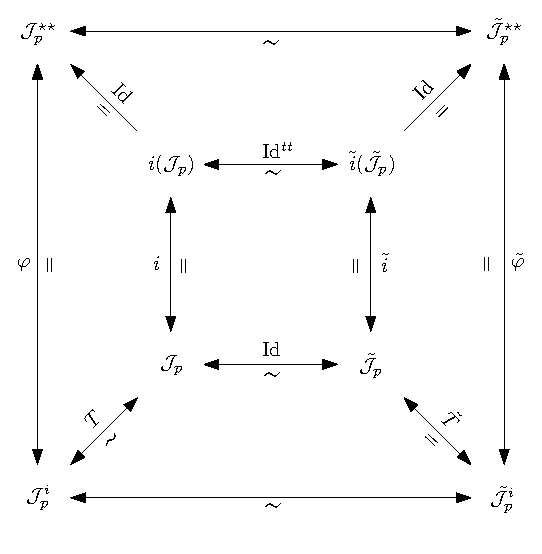
\includegraphics[width = 8.9cm,height=8.9cm]{james/isometrie.eps}}
\end{tabular}

\chapterref 

Ce chapitre prend sa source dans l'exercice 7 laiss� par Bernard Beauzamy, dans le chapitre sur les bases de Schauder (voir \cite[p. 97]{BEAUZAMY}). La section concernant la norme rendant l'espace de James isom�trique � son bidual est inspir�e de l'article de Robert Clarke James (voir \cite{JAMESISO}).
